\documentclass{article}
\usepackage[utf8]{inputenc}
\usepackage[margin=1in]{geometry}

\title{PS6}
\author{Daniel Carpenter}
\date{February 2020}

\usepackage{natbib}
\usepackage{graphicx}

\begin{document}

\maketitle

\section{Summary of Steps to Cleaning Data}
    To create the three graphs that I have posted to GitHub, I needed to pull in stock data from Yahoo Finance, \\
    which I outlined in PS5. Next, I began combining the data sets and removing excess variables. If I want to \\
    create a portfolio optimization model for my project, then I will need to combine the variables to run \\
    calculations more efficiently.
    
\section{Detailed Steps to Cleaning Data}
    \subsection{Mutate all data sets to become a data frame}
        In order to do any calculations, I first mutated all data sets into a data frame.
        
    \subsection{Create Index Column}
        Yahoo Finance does not give a date variable for their stock history, so I needed to create an index \\
        so that all three stocks aligned. If I use this data source for my project, then I will attempt to \\
        create a date variable.
        
    \subsection{Merge All Stock Variables}
        As mentioned in the summary section, I used the "merge" function in tidyverse to combine the two \\
        date sets. I used the index column that I created to join the three stocks. 
        
    \subsection{Select only needed Variables}
        In most portfolio optimization calculations, we typically only look at the "Adjusted Close" price. \\
        I only selected those columns for the three respective stocks.
        
    \subsection{Renaming Variables}
        Finally, I renamed the variables so that it only showed the stocks' ticker symbol. I did not want \\
        to type ".Adjusted" if I did not have too.
\newpage

\section{Visualizations of Market Index and Stocks}
    \subsection{What are these Visualizations Communicating?}
        These visualizations show price history over two years for the stocks. This information shows the \\
        viewer that their is great returns to be had within these money markets, which could inform them \\
        to create analysis to optimize these allocations.

    \begin{figure}[htp]
        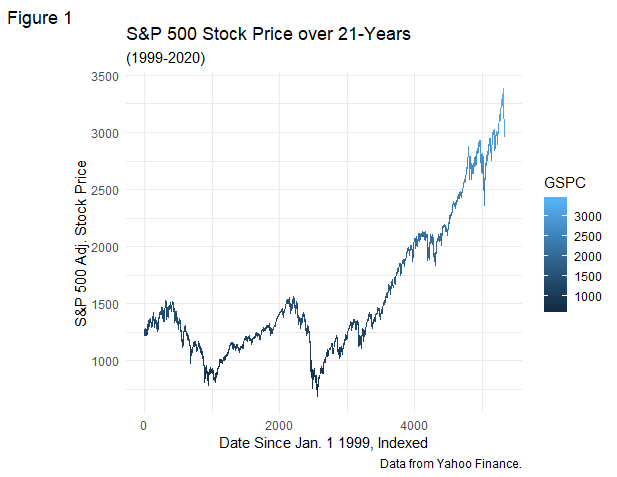
\includegraphics[width=17cm]{PS6a_Carpenter.png}
    \end{figure}
    \newpage
    
    \begin{figure}[htp]
        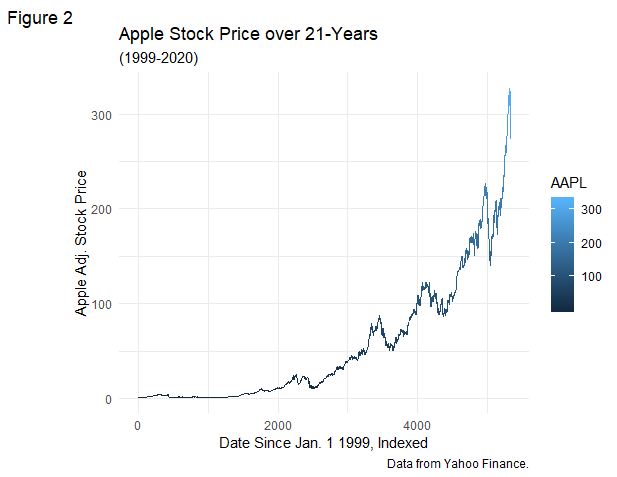
\includegraphics[width=17cm]{PS6b_Carpenter.png}
    \end{figure}
    \newpage

    \begin{figure}[htp]
        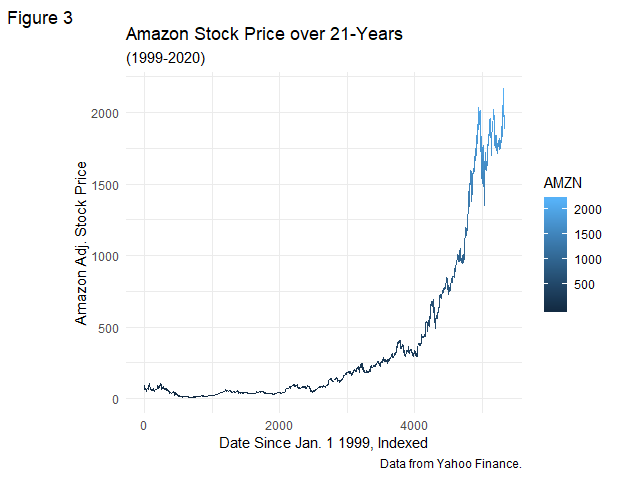
\includegraphics[width=17cm]{PS6c_Carpenter.png}
    \end{figure}

\end{document}